\section{Results} \label{sec:results}
In order to investigate how \xQ{} performs on a more realistic scenario the VIP escort problem introduced in Sec.~\ref{sec:vip_escort}. While the original escort problem is defined as a POMDP with, here we investigate a somewhat simpler version of the problem, and instead use fully observable MDPs. This is reasonable because \xQ{} operates on reward distributions, which are produced by policies on any decision making problem. The benefit of using MDPs is that they are computationally less burdensome than POMDPs, while still enabling complex decision making.

In order to find a policy for the MDP, a Monte-Carlo Tree Search (MCTS) solver will be used. As the name suggests MCTS involves building a tree from the starting state of the UGV and simulating a specified number of actions into the future and calculates the utility of each state. This process is repeated many times, and the utilities of each state are updated after each iteration of search. The actions selected by MCTS are based not only on the current utility of the state, but an exploration parameter that helps ensure that the search doesn't simply exploit the greatest known utilities. An MCTS solver is convenient to use during these experiments because the quality of the solver can be changed by modifying the parameters.

\begin{figure}[tbp]
    \centering
    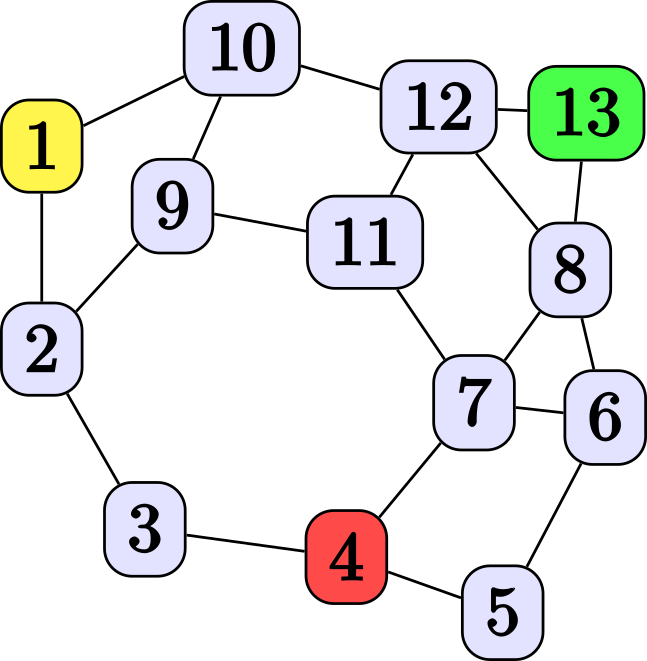
\includegraphics[width=0.4\linewidth]{Figures/original_roadnet.png}
    \caption{Diagram of the `Road Network' layout. Node 1 (yellow) is the start location of the UGV. Node 4 (red) is the start location of the pursuer vehicle. Node 13 (green) is the exit node.}
    \label{fig:roadnet}
\end{figure}

The road network is represented as shown in Fig.~\ref{fig:roadnet}. The UGV begins at the yellow node (node 1), the pursuer begins at the red node (node 4), and the desired exit is indicated by the green node (node 13). The problem is defined by the following parameters:

\tymin=80pt
\begin{table}[]
\footnotesize
\caption{Table of parameters for the VIP escort problem}
\begin{tabulary}{\linewidth}{CL}
\hline
Parameter    & Description\\
\hline
p_{trans}    & The transition probability of the UGV. This is the probability that the UGV will move in the desired direction when attempting to move. There is a probability of $1-t_prob$ that it will go to a different neighboring cell. \\
d            & MDP discount factor\\
N            & The number of nodes included in the road\\
% Mean Degree  & The target mean degree to which random networks are generated\\
e_{mcts}     & The exploration constant parameter of the MCTS.\\
d_{mcts}     & The depth of the MCTS tree\\
its_{mcts}   & The number of Monte-Carlo simulations to run to find the policy\\
rwd_{exit}   & The reward for the UGV successfully exiting the road network\\
rwd_{caught} & The reward for the UGV being caught by the pursuer\\
rwd_{sense}  & The reward for making a movement
\hline
\end{tabulary}
\end{table}
\begin{table*}
    \footnotesize
    \centering
    \caption{Parameters used for the different experiments}
    \label{tab:exps}
    \begin{tabular}{llcccccccccc} \toprule
        &\multicolumn{10}{c}{Parameters} \\ \cmidrule(r){3-12}
        \#  & Variable(s) & Network &p_{trans}&d&N&e_{mcts}&d_{mcts}&its_{mcts}&rwd_{exit}&rwd_{caught}&rwd_{sense} \\ \midrule
        1 & \{d_{mcts}\} & Fig.~\ref{fig:roadnet} & $[0.0,1.0]$ & $0.95$ & 13 & $[1000.0]$ & [1:1:10] & 1000 & 2000 & -2000 & -100\\
        2 & \{d_{mcts}\} & Fig.~\ref{fig:med_roadnet} & $[0.0,1.0]$ & $0.95$ & 45 & $[1000.0]$ & [1:3:28] & 1000 & 2000 & -2000 & -100\\
        3 & \{p_{trans}\}& Fig.~\ref{fig:roadnet} & $[0.0,1.0]$ & $0.95$ & 13 & $[1000.0]$ & [8,3,1] & 1000 & 2000 & -2000 & -100\\
        4 & \{p_{trans},e_{mcts}\} & Fig.~\ref{fig:roadnet} & $[0.0,1.0]$ & $0.95$ & 13 & $[10.0,1000.0]$ & [8,3,1] & 1000 & 2000 & -2000 & -100\\
    \end{tabular}
\end{table*}

Three experiments were run. First, \xQ{} was calculated for MCTS solvers of different depth on the network from Fig.~\ref{fig:roadnet} (all other parameters were held constant). Second, \xQ{} was evaluated for a candidate solver for different values of $p_{trans}$. Finally, \xQ{} was evaluated for a candidate solver at different $p_{trans}$ and $e_{mcts}$.

\subsection{Varying $d_{mcts}$}
This investigation involved experiments 1 and 2 from Table~\ref{tab:exps}. The MCTS solver was run on each of the two networks ($N=13$ for 1, and $N=45$ for 2) with different depths. In each case one of the solvers was chosen as the trusted one (i.e. chose a `good' solver, but not necessarily the `best' one). In the case of experiment 1 that was the $d_{mcts}=9$ solver, and in experiment 2 it was the $d_{mcts}=25$ solver.

\begin{figure}[tbp]
    \centering
    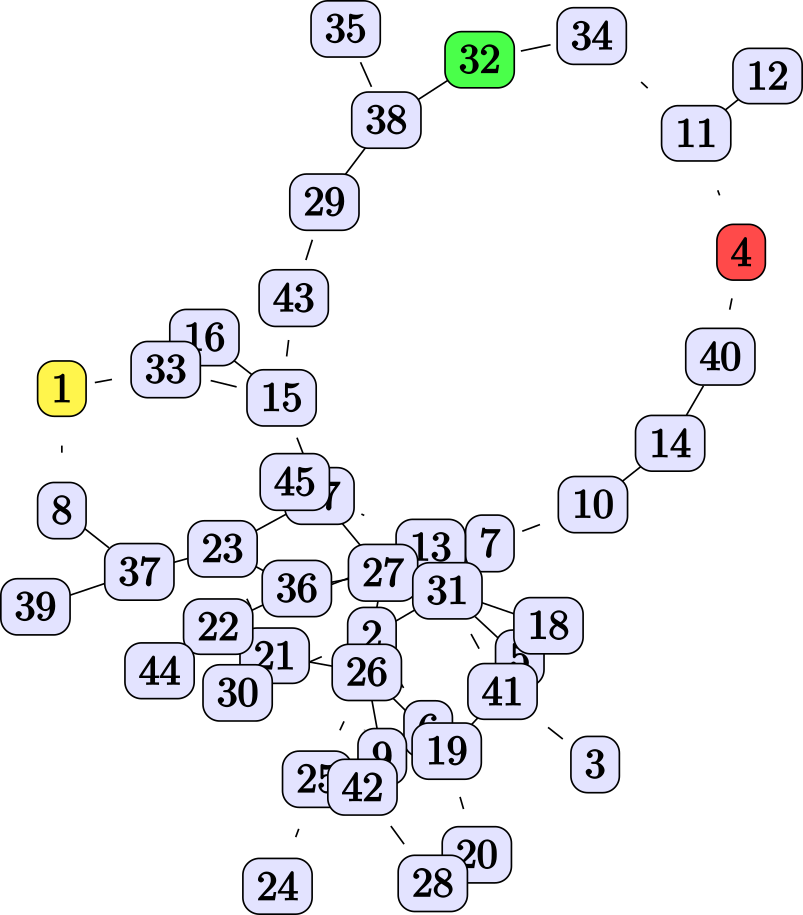
\includegraphics[width=0.4\linewidth]{Figures/medium_roadnet.png}
    \caption{Diagram of a randomly generated road network with that is quite a bit larger ($N=45$) than the original shown in Figure \ref{fig:roadnet}.}
    \label{fig:med_roadnet}
\end{figure}

In this case we choose the trusted solver to be a MCTS solver with $N=1000$, $D=8$, and $e=1000.0$. For the road network, the transition probability is $p=0.8$ (which means the UGV will travel to the intended location $80\%$ of the time, and a different direction the other $20\%$ of the time). The reward distributions are obtained by running 250 simulations using the same initial conditions.

\begin{figure}[tbp]
    \centering
    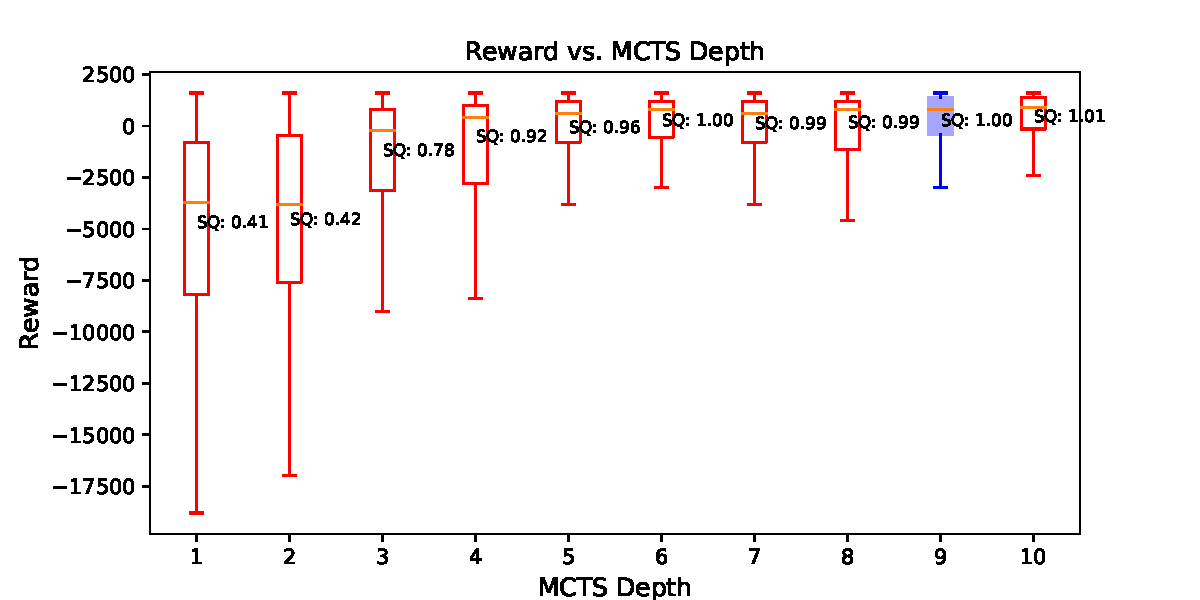
\includegraphics[width=1.0\linewidth]{Figures/sq_roadnet_mcts_i100e1000.pdf}
    \caption{Varying the MCTS `D' parameter for the road network in Figure \ref{fig:roadnet}. Here the solver is using $N=100$ iterations, and an exploration constant of $e=1000$. The \xQ{} values being calculated are with respect to the trusted distribution highlighted, which in this case is the solver with depth equal 9.}
    \label{fig:mcts_d}
\end{figure}
\begin{figure}[tbp]
    \centering
    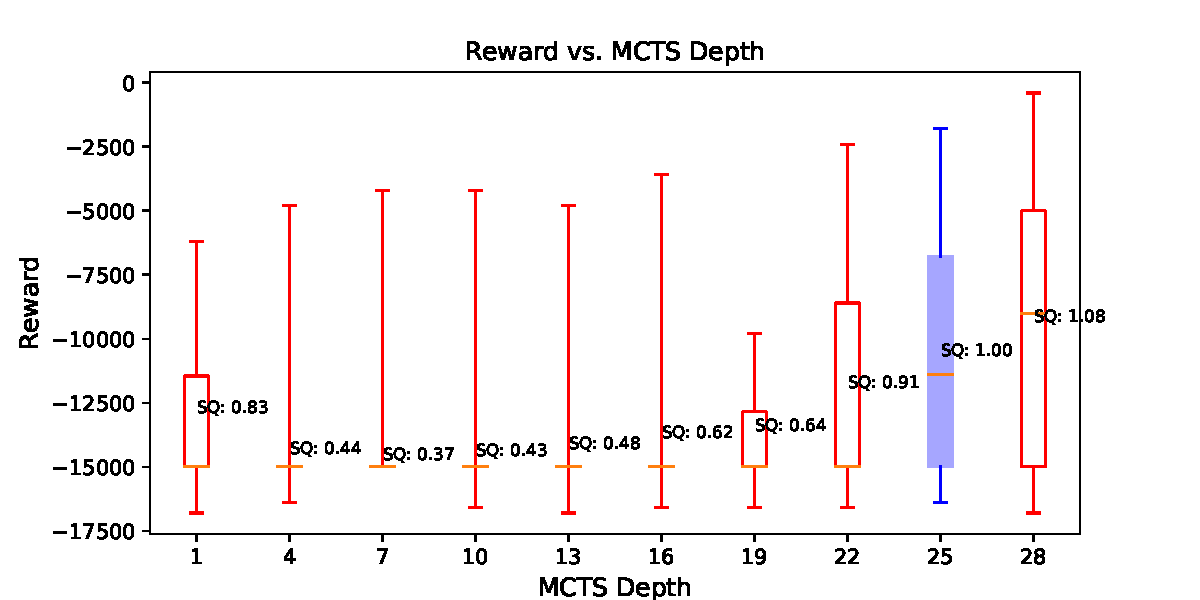
\includegraphics[width=1.0\linewidth]{Figures/sq_mednet_mcts_i1000e2000.pdf}
    \caption{Varying the MCTS `D' parameter for the road network in Figure \ref{fig:med_roadnet}. Here the solver is configured using $N=1000$ iterations and an exploration constant of $e=2000$.}
    \label{fig:mcts_d_med}
\end{figure}


\subsection{Varying the transition probability}
In this case a solver quality model was trained using a `trusted' MCTS solver with:

\begin{figure}[tbp]
    \centering
    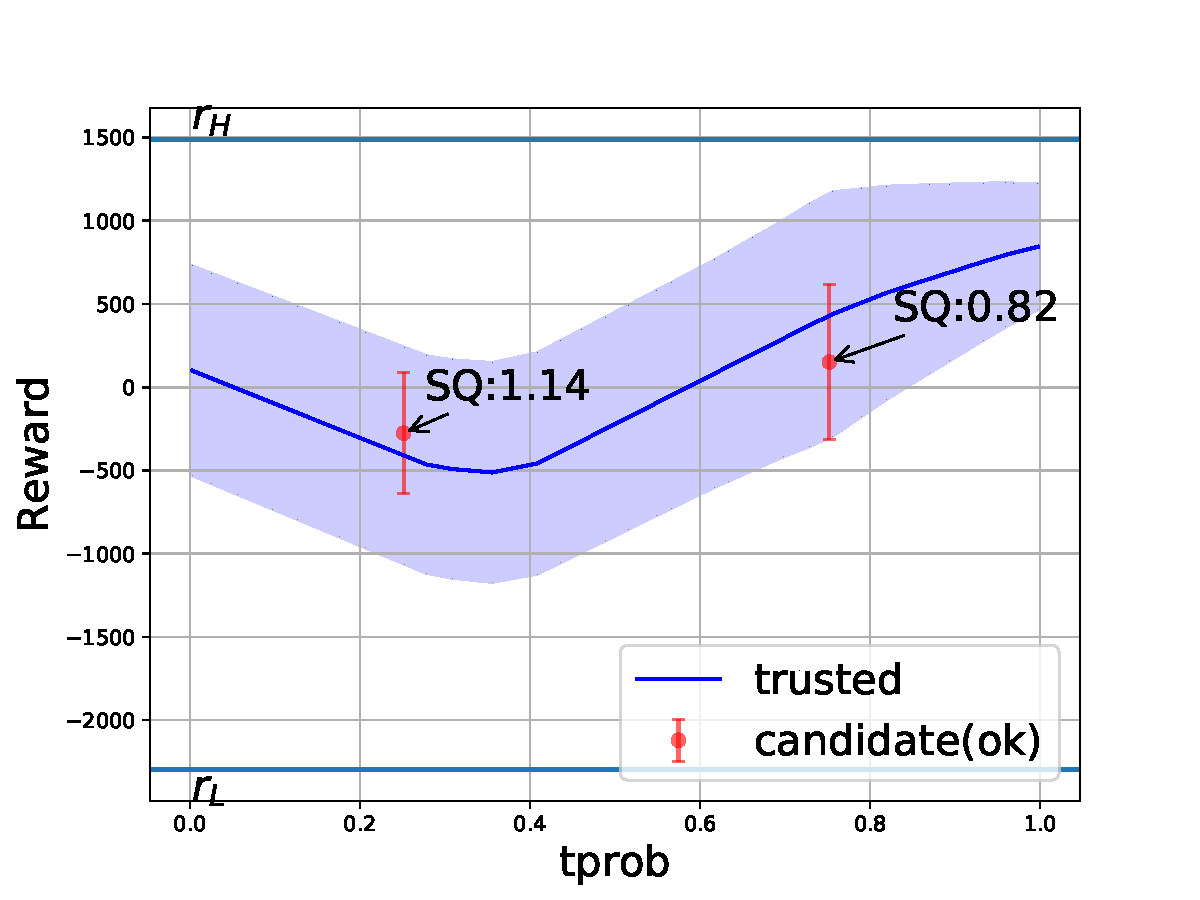
\includegraphics[width=0.9\linewidth]{Figures/transition_vary_tprob_ok.pdf}
    \caption{Using a solver with depth 3}
    \label{fig:tprob}
\end{figure}
\begin{figure}[tbp]
    \centering
    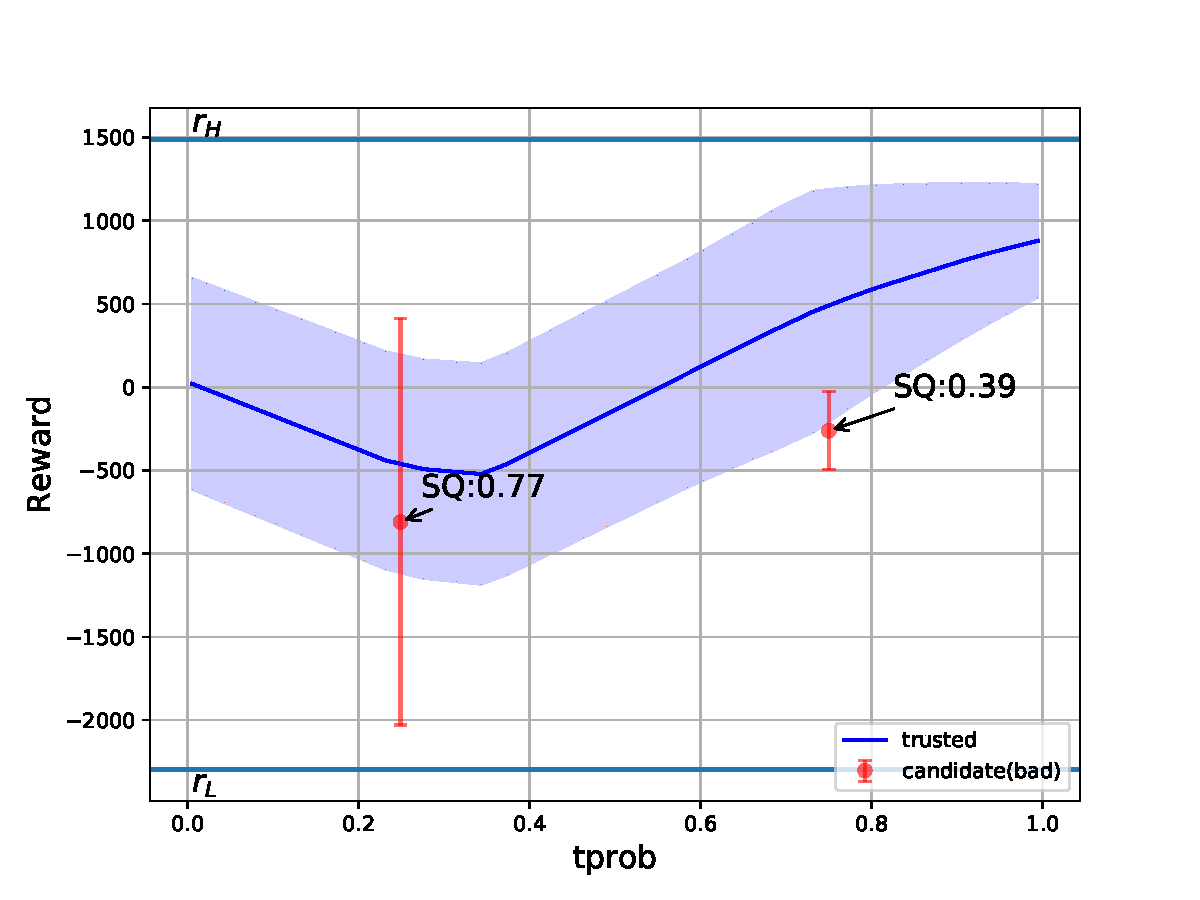
\includegraphics[width=0.9\linewidth]{Figures/transition_vary_tprob_bad.pdf}
    \caption{Using a solver with depth 1}
    \label{fig:tprob}
\end{figure}

\subsection{Varying the transition probability and exploration constant}

\begin{figure}[tbp]
    \centering
    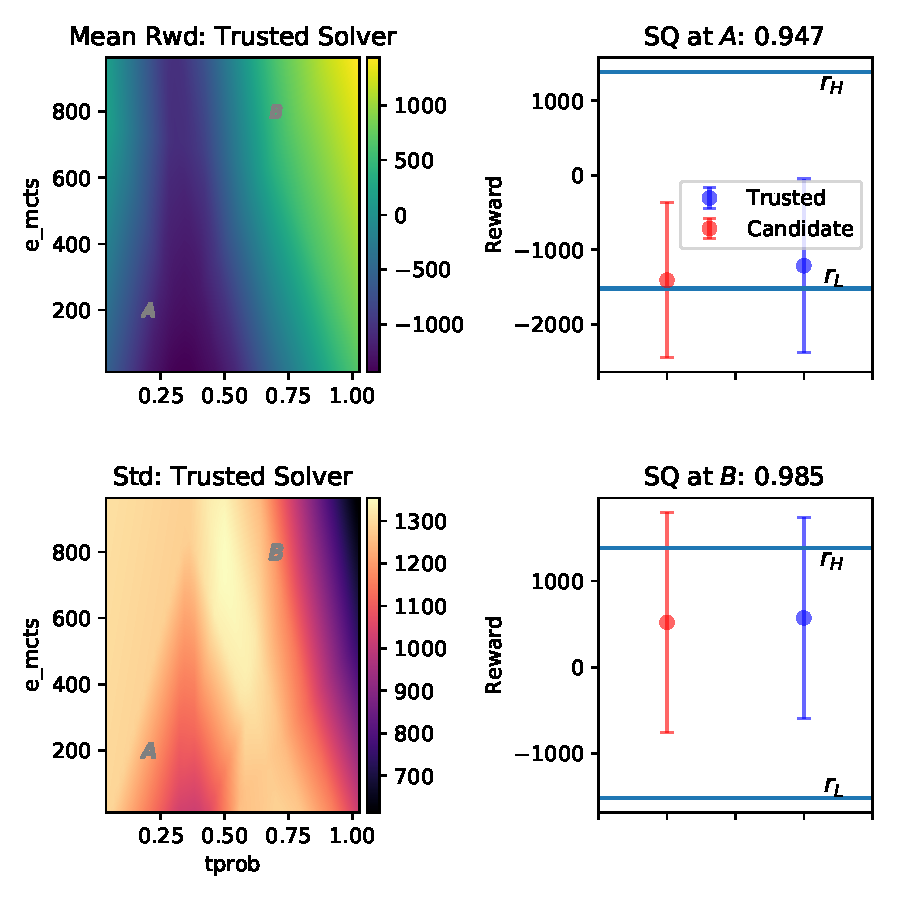
\includegraphics[width=0.9\linewidth]{Figures/transition_e_vary_e_mctstprob_ok.pdf}
    \caption{using a solver with depth 3}
    \label{fig:tprob}
\end{figure}
\begin{figure}[tbp]
    \centering
    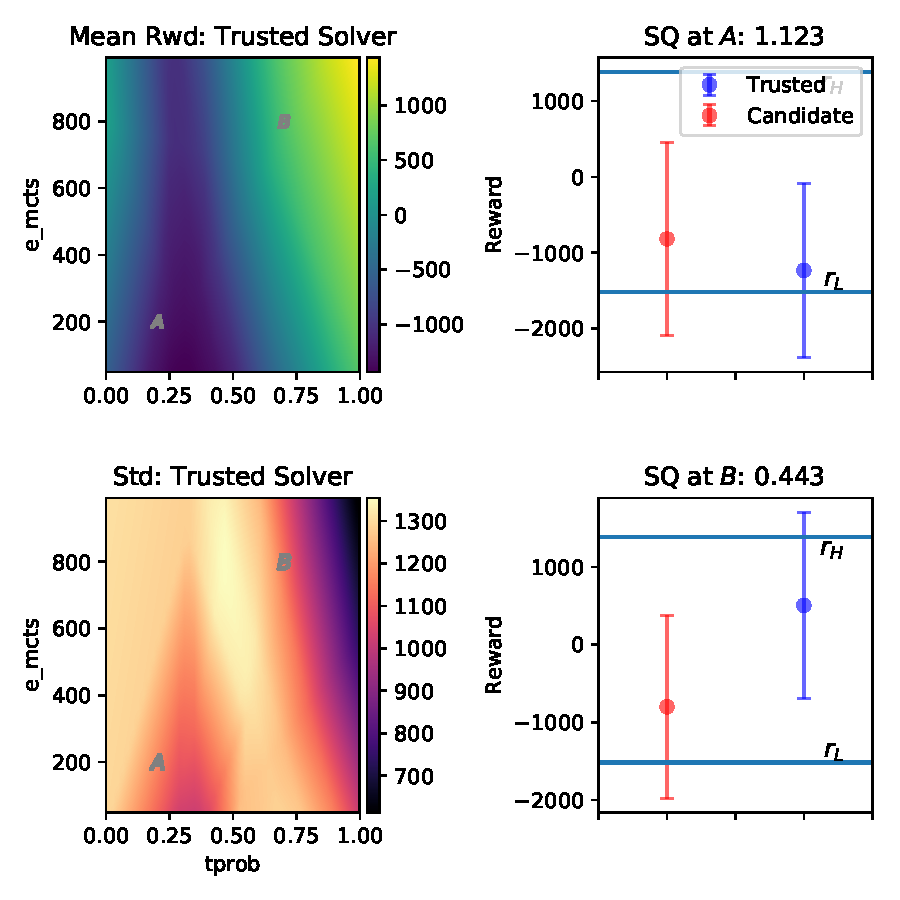
\includegraphics[width=0.9\linewidth]{Figures/transition_e_vary_e_mctstprob_bad.pdf}
    \caption{Using a solver with depth 1}
    \label{fig:tprob}
\end{figure}
